% Fig. 3.24 -- the smallest order statistic Y_1 splits the support into two
%   stretches: none of the sample lies to its left, the other n-1 lie to its
%   right.
% Source: mathstatch3.tex lines 5272-5286.  Manuscript geometry kept: a
%   number line 0 to 10 with an arrow at the right end, a divider at x = 3
%   named y_1, the counts above the line at x = 1.5 and x = 6.5, and two
%   dashed arcs under the line spanning 0 to 3 and 3 to 9.95, labelled with
%   the probability that one sample value falls in that stretch.
%
% First of the four-figure series 3.24-3.27; all four share this file's
% coordinates, divider height, arc depth and type size, so that they read as
% one series.
%
% Departures from the manuscript picture:
%
% 1. The manuscript writes the counts as "0 個" and "n-1 個".  Chinese cannot
%    be set by this pipeline (spec 1.4), so the counts are left as bare
%    mathematics above each stretch and the caption says what they count.
%
% 2. The manuscript hangs y_1 under the axis at (3,-0.1).  The two arcs meet
%    at (3,0) and climb away from it at a slope of 0.53, so a label there sits
%    0.05cm from the left arc, against the 0.18cm clearance of spec 1.3.  The
%    label is therefore carried at the top of the divider, which leaves the
%    whole of the space under the line to the arcs and their labels.  Same
%    change in the other three figures of the series.
%
% 3. The manuscript draws the arcs with TikZ's "bend right" (30 degrees for
%    the short one, 14 for the long one), whose sag grows with the span: over
%    this figure it comes out at 0.375 and 0.420 units, and in Fig. 3.26,
%    where both arcs are long and both angles are left at 30, at 0.62.  The
%    arcs are drawn here as explicit cubics with control points at one third
%    of the span and ordinate -4/3 x 0.40, which sets the sag of every arc of
%    the series to exactly 0.40 units.
%
% 4. F_{\sssig X} of the manuscript is written F_X inside the picture, per
%    CH3_FIGURE_SPECS.md section 6: \scriptscriptstyle would drop the
%    subscript to 8pt at the size used here.  The symbol is unchanged.
%
% \DeclareMathSizes{10}{10}{9}{8} raises the math script sizes from the
% default 7pt/5pt, as in quartiles-equal-areas.tex.  Native width 249.343pt
% (drawing range 8.63cm, inside the 9.0cm cap of spec 1.3).  A mark of S pt
% shows at S x 0.99626 x <display width> / 249.343 px, so in a
% topic-figure--wide at the 350px phone width
%     10pt text 13.98px, 9pt scripts 12.59px
% and at the 620px desktop width 24.77 / 22.30px.  The smallest marks in the
% picture are the X of F_X and the 1 of y_1, both at script size.
\documentclass[tikz,border=2pt]{standalone}
\usepackage{amsmath}
\usepackage{amssymb}
\usepackage{xcolor}
\usetikzlibrary{arrows.meta}
\DeclareMathSizes{10}{10}{9}{8}

\definecolor{journalink}{HTML}{1F1C18}
\definecolor{journalmuted}{HTML}{8A7F72}
\definecolor{journalaccent}{HTML}{9C2D2D}

\begin{document}
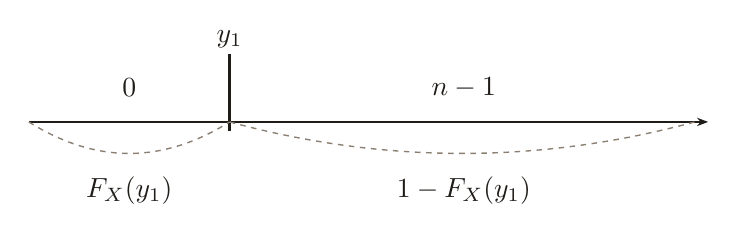
\begin{tikzpicture}[
  x=0.85cm,
  y=1cm,
  every node/.style={font=\normalsize, journalink, inner sep=1pt},
  axis/.style={journalink, line width=0.8pt, -{Stealth[length=4pt]}},
  divider/.style={journalink, line width=0.8pt},
  arc/.style={journalmuted, line width=0.5pt, dash pattern=on 2pt off 2pt}
]
  % ---- the number line -------------------------------------------------
  \draw[axis] (0,0) -- (10.15,0);

  % ---- the cut at y_1 --------------------------------------------------
  \draw[divider] (3,-0.12) -- (3,0.86);
  \node[anchor=south] at (3,0.90) {$y_1$};

  % ---- how many of the sample lie in each stretch ----------------------
  \node at (1.5,0.43) {$0$};
  \node at (6.5,0.43) {$n-1$};

  % ---- the probability of each stretch ---------------------------------
  % Cubics of sag 0.40: control points at one third of the span, ordinate
  % -4/3 x 0.40 = -0.5333, since the midpoint of such a cubic sits at 3/4 of
  % the control ordinate.
  \draw[arc] (0,0) .. controls (1,-0.5333) and (2,-0.5333) .. (3,0);
  \draw[arc] (3,0) .. controls (5.3167,-0.5333) and (7.6333,-0.5333)
    .. (9.95,0);
  \node[anchor=north] at (1.5,-0.65) {$F_X(y_1)$};
  \node[anchor=north] at (6.5,-0.65) {$1-F_X(y_1)$};
\end{tikzpicture}
\end{document}
